% ****** Start of file apssamp.tex ******
%
%   This file is part of the APS files in the REVTeX 4.1 distribution.
%   Version 4.1r of REVTeX, August 2010
%
%   Copyright (c) 2009, 2010 The American Physical Society.
%
%   See the REVTeX 4 README file for restrictions and more information.
%
% TeX'ing this file requires that you have AMS-LaTeX 2.0 installed
% as well as the rest of the prerequisites for REVTeX 4.1
%
% See the REVTeX 4 README file
% It also requires running BibTeX. The commands are as follows:
%
%  1)  latex apssamp.tex
%  2)  bibtex apssamp
%  3)  latex apssamp.tex
%  4)  latex apssamp.tex
%
\documentclass[%
 reprint,
%superscriptaddress,
%groupedaddress,
%unsortedaddress,
%runinaddress,
%frontmatterverbose, 
%preprint,
%showpacs,preprintnumbers,
%nofootinbib,
%nobibnotes,
%bibnotes,
 amsmath,amssymb,
 aps,
%pra,
%prb,
%rmp,
%prstab,
%prstper,
%floatfix,
]{revtex4-1}

\newcommand{\partDeriv}[2]{\frac{\partial #1}{\partial #2}}

\usepackage{graphicx}% Include figure files
\usepackage{dcolumn}% Align table columns on decimal point
\usepackage{bm}% bold math
%\usepackage{hyperref}% add hypertext capabilities
%\usepackage[mathlines]{lineno}% Enable numbering of text and display math
%\linenumbers\relax % Commence numbering lines

%\usepackage[showframe,%Uncomment any one of the following lines to test 
%%scale=0.7, marginratio={1:1, 2:3}, ignoreall,% default settings
%%text={7in,10in},centering,
%%margin=1.5in,
%%total={6.5in,8.75in}, top=1.2in, left=0.9in, includefoot,
%%height=10in,a5paper,hmargin={3cm,0.8in},
%]{geometry}

\begin{document}

%\preprint{APS/123-QED}

\title{On The Diffusion of Sticky Particles in 1-D}% Force line breaks with \\
%\thanks{A footnote to the article title}%

\author{Joshua DM Hellier}
 \email{J.D.M.Hellier@sms.ed.ac.uk}
% \altaffiliation[Also at ]{Physics Department, XYZ University.}%Lines break automatically or can be forced with \\
\author{Graeme J Ackland}%
 \email{G.J.Ackland@ed.ac.uk}
\affiliation{%
 SUPA, School of Physics and Astronomy, University of Edinburgh, Mayfield Road, Edinburgh EH9 3JZ, United Kingdom
}%

%\collaboration{\noaffiliation}

%
%\author{Charlie Author}
% \homepage{http://www.Second.institution.edu/~Charlie.Author}
%\affiliation{
% Second institution and/or address\\
% This line break forced% with \\
%}%
%\affiliation{
% Third institution, the second for Charlie Author
%}%
%\author{Delta Author}
%\affiliation{%
% Authors' institution and/or address\\
% This line break forced with \textbackslash\textbackslash
%}%

%\collaboration{CLEO Collaboration}%\noaffiliation

\date{\today}% It is always \today, today,
             %  but any date may be explicitly specified

\begin{abstract}
This is where I would write the abstract. This is probably best left until the end, as then I'll know what I'm actually summarising.
\iffalse
\begin{description}
\item[Usage]
Secondary publications and information retrieval purposes.
\item[PACS numbers]
May be entered using the \verb+\pacs{#1}+ command.
\item[Structure]
You may use the \texttt{description} environment to structure your abstract;
use the optional argument of the \verb+\item+ command to give the category of each item. 
\end{description}
\fi
\end{abstract}

%\pacs{Valid PACS appear here}% PACS, the Physics and Astronomy
                             % Classification Scheme.
%\keywords{Suggested keywords}%Use showkeys class option if keyword
                              %display desired
\maketitle


\section{Introduction} \label{sec:intro}
There are a great many natural phenomena which involve the diffusion of small particles through solids; interface problems, such as the growth of a titanium dioxide layer on the surface of titanium metal exposed to air, are good examples~\cite{tegner2015high}.
If we wish to answer questions such as why these interfaces grow, or how quickly, we really need to understand how particles diffuse through crystal lattices, especially in the case when they interact with each other.
In this paper we will introduce a very simple locally interacting exclusion model of this kind of diffusion, and we will explore the continuum-level implications of such a model.

We would intuitively expect that our titanium interface growth problem would involve the diffusion of oxygen atoms through titanium metal crystals. Once the concentration of oxygen is high enough, the medium becomes titanium dioxide.
The oxygen atoms do this primarily by hopping between the interstitial sites between the titanium atoms.
% Need citation
It is extremely energetically unfavourable for multiple oxygen atoms to occupy such a site,
%citation needed
therefore to a good approximation we may regard these oxygen atoms as excluding each other from these sites, just like in ASEP~\cite{sugden2007dynamically, liggett1985interacting}.

Next, let us assume that the lattice that the oxygen atoms move through is fairly rigid\footnote{I.e. that the titanium atoms are quite tightly bound and don't move that much, which is reasonable as they are metal atoms in a metal.},
and that the interactions between the oxygen atoms are quite short-ranged\footnote{Any electrostatic forces should be rapidly screened by the metal, thus the main interaction should be via short-range electrostatics and electron sea distortion.}.
Finally, we should note that even though a problem like interface growth happens in three-dimensional space, the problem is rotationally and translationally invariant in a plane perpendicular to the direction of growth; therefore the
interesting aspects of the problem are one-dimensional. Indeed, in anisotropic solids it is often the case that diffusion occurs much more rapidly along parallel chains than in other directions.

Putting these assumptions together, we are motivated to investigate the model described by the rates detailed in Figure~\ref{fig:rates}. It is essentially the symmetric exclusion model, only now the presence of an adjacent particle
causes the hopping rate to change. We will henceforth refer to the model as the ``sticky hopping model'', or SHM.
\begin{figure}[h!]
\vspace{1em}
\label{fig:rates}
 \begin{tabular}{c@{\hspace{1em}}c@{\hspace{1em}}c@{\hspace{1em}}c}
    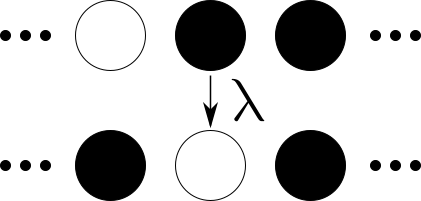
\includegraphics[width=0.22\linewidth]{../tex-src/images/rates4} & 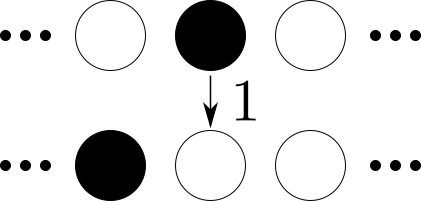
\includegraphics[width=0.22\linewidth]{../tex-src/images/rates1} & 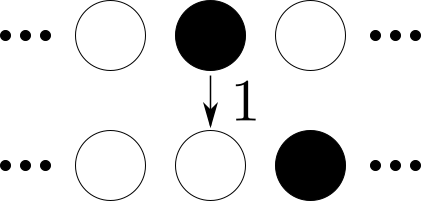
\includegraphics[width=0.22\linewidth]{../tex-src/images/rates2} & 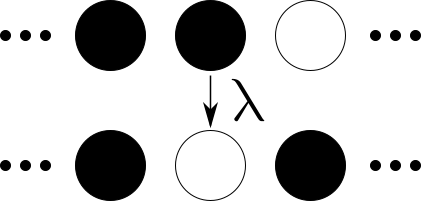
\includegraphics[width=0.22\linewidth]{../tex-src/images/rates3} \\
    \end{tabular}
    \vspace{-1em}
\caption{Filled circles indicate particles, empty circles indicate empty sites (vacancies). Particles randomly move into adjacent vacancies with rate $1$ (having rescaled time for notational convenience), unless there is a particle behind the position they're moving from,
in which case they move with rate $\lambda$; $\lambda<1$ represents attractive forces between particles, and $\lambda>1$ repulsive.}
\end{figure}


\section{Model Phenomenology}
The model described in Figure~\ref{fig:rates} is very simple, but numerical simulation shows that it is capable of a wide range of behaviours, such as those shown in Figures~\ref{fig:eyeCandy} and ~\ref{fig:flowTable}. We will discuss
these numerical results in more detail in Section~\ref{sec:numRes}, but first let us try to predict the model behaviour using analytic means.

\subsection{Mean-Field Theory Derivation}
Let the spacing between lattice sites be $a$, $\tau_0$ be the non-sticky hopping timescale and the time-averaged\footnote{Or ensemble-averaged, assuming ergodicity.} occupation probability of the $i^{\mathrm{th}}$ lattice site be $\rho_i$. 
One may show that, in the mean-field approximation regime,
\begin{align*}
 \tau_0 \partDeriv{\rho_i}{t} = &\left( 1-\rho_i \right) \left[ \left(1-\zeta\rho_{i-2} \right) \rho_{i-1} + \left(1-\zeta\rho_{i+2} \right) \rho_{i+1} \right] \\
 &- \rho_i \left[ 2 \zeta \rho_{i-1} \rho_{i+1}  - (3-\zeta)\left(\rho_{i-1} + \rho_{i+1}\right) + 2 \right],\\
\end{align*}
where $\zeta = 1-\lambda$ is to be regarded as a ``stickiness parameter''. Switching to the continuum limit by taking $a\rightarrow 0$, and neglecting $\mathcal{O}(a^4)$ terms, we may reexpress this as a conserved flow $J$ as follows:
\begin{align*}
 \partDeriv{\rho}{t} &= - \partDeriv{J}{x}, \\
 J &= - \frac{a^2}{\tau_0} A(\rho) \partDeriv{\rho}{x}, \\
 A &= 1 - \zeta \rho(4-3\rho). \\
\end{align*}
Thus, the MFT says that the particles should diffuse with a diffusion coefficient which depends upon the local density.
\subsection{Continuum MFT Predictions}
First let us consider some limits. As $\zeta \rightarrow 0$ (in other words, as the model becomes a simple exclusion model), $A \rightarrow 1$, so the MFT smoothly changes to match the known result. Likewise, in the
dilute limit $\rho \rightarrow 0$, $A \rightarrow 1$, reflecting the fact that it becomes a dilute lattice gas and therefore the interactions between particles become irrelevant as they never meet.
Conversely, in the full limit $\rho \rightarrow 1$, $A \rightarrow \lambda$; this makes sense because we now have a dilute gas of vacancies, which hop with rate $\lambda$.
One may observe that the continuum limit MFT has a symmetry under $\rho \mapsto \frac{4}{3} - \rho$; thus, the dynamics should be symmetric under a density profile reflection around $\rho = \frac{2}{3}$. This is where $A$ always
attains its extremal value, $ 1 - \frac{4}{3}\zeta$, hence for $\zeta>3/4$ the diffusion coefficient becomes negative in regions with
$\frac{2}{3} - \frac{\sqrt{\zeta\left(4\zeta - 3\right)}}{3\zeta} \textless \rho \textless \frac{2}{3} + \frac{\sqrt{\zeta\left(4\zeta - 3\right)}}{3\zeta}$.
Finally, it is possible to show that solutions to the continuum MFT containing domains with negative a negative diffusion coefficient are linearly unstable.
\subsection{MFT Solutions}
\subsubsection{Steady-State Flow Through a Block}
It is possible to solve the continuum MFT in a steady state on a finite domain, say $x\in(0, L)$. The continuity equation implies that $J(x)=J_0$, and by integrating both sides of our current equation with respect to $x$ we find that
\begin{equation}
 J_0 (x-x_0) = -\frac{a^2}{\tau_0} \rho \left(1+\zeta \rho\left(\rho-2\right)\right),
\end{equation}
a cubic equation which can be solved to give $\rho(x)$. If we impose Dirichlet boundary conditions on this system, say $\rho(0)=\rho_0$ and $\rho(L)=\rho_L$, we find that
\begin{equation}
 J = \frac{a^2}{L \tau_0} \left[ \rho_0 - \rho_L + \zeta \left( \rho_0\left(\rho_0^2-2\right) - \rho_L\left(\rho_L^2-2\right) \right) \right].
\end{equation}
We may consider applying small concentration gradients across a block by setting $\rho_0 = \rho_M + \frac{1}{2}\delta\rho$ and $\rho_L = \rho_M - \frac{1}{2}\delta\rho$. Doing so, we find that
\begin{equation}
\label{eq:MFTflow}
 \partDeriv{J}{\delta\rho}\bigg|_{\delta\rho=0} = \frac{a^2}{L \tau_0} \left[ 1 - \zeta\rho_M(4-3\rho_M) \right],
\end{equation}
a result we will make use of when we come to analyse our numerics in Section~\ref{sec:numRes}.
\subsubsection{Constant Speed Solution}
According to Ivanova~\cite{ivanova2007}, we can have travelling solutions to our time-dependent MFT PDE. Introducing the variable $\omega = x - vt$, with $v\in \mathbb{R}$, our PDE solution $\rho(x, t) = \phi(\omega)$ obeys
\begin{equation}
 v \phi ' = -\frac{a^2}{\tau_0} \left[ 1-\zeta \phi \left(4-3\phi\right) \right] '
\end{equation}
with general solution found by solving
\begin{equation}
 \omega = \frac{a^2}{\tau_0 v} \left[ \frac{1}{2} \zeta \phi \left(8-6\mu-3\phi\right) - \left(1-\zeta\left(4-3\mu\right)\mu\right) \log{\left(\phi-\mu\right)} \right].
\end{equation}
Requiring that $\phi \rightarrow  1$ as $\omega \rightarrow 0$ and $\phi \rightarrow 0$ as $\omega \rightarrow \infty$, this reduces to
\begin{equation}
 \omega = \frac{a^2}{\tau_0 v} \left[ \frac{1}{2} \zeta \phi \left(8-3\phi\right) - \log{\left(\phi\right)} - \frac{5 \zeta}{2} \right],
\end{equation}
so at the leading edge of the wave, $\omega \rightarrow \infty$, $\phi \sim e^{-\frac{v \omega}{a^2}} $. At $\omega \rightarrow 0$ with $\phi \rightarrow 1$, which would physically represent the interface between the particle-saturated
region and the non-saturated region, $\phi \sim 1 - \frac{v \omega}{a^2 \lambda}$. Note that the value of $v$ is not restricted by these equations, and a linear stability analysis of the leading edge does not imply speed selection like in
the case of the Fisher wave\cite{sherratt1998transition}, so it seems like the speed of travelling wavefronts would be determined by the initial conditions; of course, we should expect the MFT to misbehave close to the interface,
so the actual system would probably have some interface-based mechanism for choosing its wave-speed.


\section{Numerical Results}
\label{sec:numRes}
We now have some MFT predictions about the SHM, and a few ideas about when those predictions might be invalid. Thus, it is prudent for us to test them out numerically.
There are a few different methods which could have been used, but I chose to calculate using the \texttt{KMCLib}\cite{leetmaa2014kmclib} package, which implements the Kinetic Monte Carlo algorithm (essentially the same as the Gillespie algorithm)
on lattice systems. \texttt{KMCLib} has the advantage that it is python-wrapped \texttt{C++}, and thus quite easy to use whilst at the same time being quite computationally efficient; thus it was fairly easy for me to carry out large numbers
of differently-parametrised serial \texttt{KMCLib} jobs on the \texttt{Eddie3} computing cluster here at Edinburgh.
\subsection{Flow in a Block}
As we have MFT predictions about flow in a block, we can try to simulate that situation using KMC. In the bulk, the transition rates are simply those described in Figure~\ref{fig:rates}. At the boundaries, referred to as the ``top'' and ``bottom''
of the block, there are 2 layers of lattice sites what switch between being full and empty with rates such that the time-averaged occupation can be specified to match the desired boundary conditions; there are then chances for particles to spawn
and despawn with rates depending upon the occupation of these boundary layers. In the end, the intention is that these boundaries should reproduce the effect of having particle reservoirs attached to the ends, which is something we can check for
sanity in the output by inspecting the time-averaged occupations of sites near the boundary.

In our calculations, we set the top and bottom densities to be $\rho_T = \rho_M - \frac{1}{2} \delta\rho$ and $\rho_B = \rho_M + \frac{1}{2} \delta\rho$ respectively, as well as specifying the value of $\lambda$ and the number of sites
in the lattice. During the calculation, we perform a specified number
of Gillespie steps, and count the number of particles entering at the top $e_T$, leaving at the top $l_T$, entering at the bottom $e_B$, leaving at the bottom $l_B$, as well as the Gillespie time interval $T$ that elapses during
those steps; we then have an estimate of the overall flow rate $J$ via
\begin{equation}
 J = \frac{e_B-e_T+l_T-l_B}{2T}.
\end{equation}
We can also count the total number of particles in the system in order to measure the average particle density, although we need to make sure that it is correctly time-averaged.
If we keep $\delta\rho$ relatively small, $J$ varies approximately linearly with $\delta\rho$; thus if we calculate $J$ for a series of small $\delta \rho$, we can perform linear regression to find $\partDeriv{J}{\delta\rho}\big|_{\delta\rho=0}$,
the effective diffusion coefficient. Computing this for different $(\rho_M, \lambda)$ combinations gives us numerical data which can be compared with the MFT result in Equation~\ref{eq:MFTflow}.
\begin{figure*}[h!]
\vspace{1em}
\caption{\label{fig:diffCoef} The contour plot on the left shows the MFT prediction of the diffusion coefficient $D=\partDeriv{J}{\delta\rho}\big|_{\delta\rho=0}$ as a function of local density $\rho_M$ and $\lambda$;
we are only plotting where $0 \le D \le 1.2$, other regions are shown in white, including the region in which $D<0$, which would cause instabilities preventing a flow from actually occurring. On the right is our numerical calculation of $D(\rho_M, \lambda)$,
with exactly the same plotting ranges. The dots indicate which points in $(\rho_M, \lambda)$ we calculated $D$ around, to give an impression of how the interpolation in the contour plot was done.}
\begin{center}
 \begin{tabular}{c@{\hspace{1em}}c}
    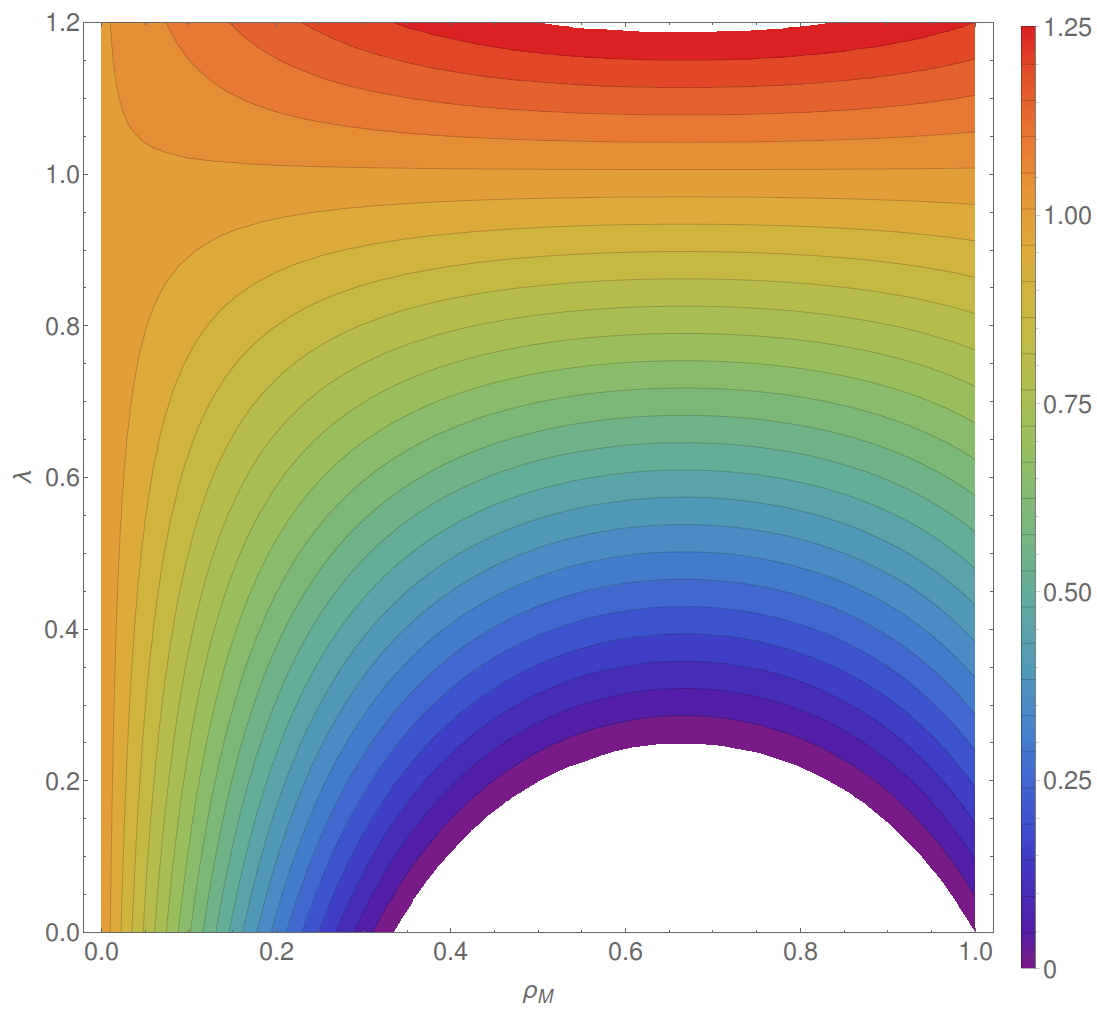
\includegraphics[width=0.5\linewidth]{../tex-src/images/analFlow.png} & 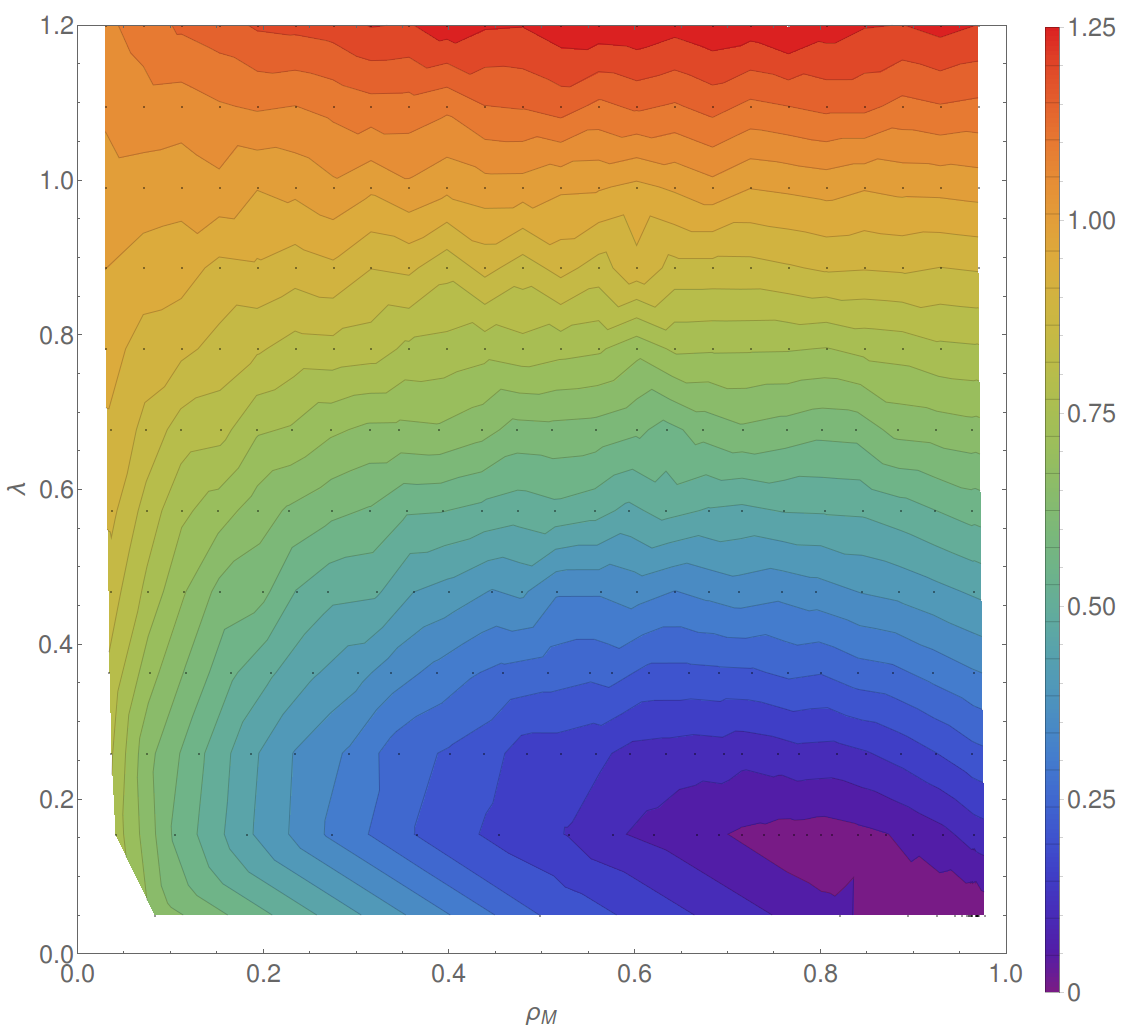
\includegraphics[width=0.5\linewidth]{../tex-src/images/dataFlow.png} \\
    \end{tabular}
\end{center}
    \vspace{-0em}
\end{figure*}
To produce the results in Figure~\ref{fig:diffCoef}, for each $(\rho_T, \rho_B, \lambda)$ combination we created the initial state by randomly inserting particles into an empty 124-length lattice, so that the density was $\rho_M$. We then ran the simulation for
$1.6\times10^8$ steps, to wash away any spurious initial-data effects and allow the system to reach a steady state flow. We then ran for $8\times10^7$ steps whilst measuring flow rate and density, then allowed the system to run for $1.6\times10^7$
steps without taking measurements in an effort to suppress temporal autocorrelation effects. This alternating process was repeated 10 times, yielding 10 measurements of flow rate and density, from which estimates of these quantities and their
standard errors could be obtained. The whole setup was repeated with a 60-length system, in order to check for edge effects; however, the results were not significantly different, so those would not seem to be a problem.

We can of course obtain estimates of the confidence interval for our linear regression coefficient, and thus generate a standard error for $\partDeriv{J}{\delta\rho}\big|_{\delta\rho=0}$; likewise we can obtain goodness of fit estimates for the
regression. I have neglected to plot them here due to space constraints, but they are in included in the additional materials.
%REMEMBER TO ACTUALLY PUT IT THERE!!!

\subsection{Flow Structure}
\label{sec:flowStruc}
It is possible to produce diagrams which show the changes in short-time-averaged local density as a function of space and time. I have made such diagrams for a selection of $(\rho_M, \lambda)$ pairs, so that the reader can
get an impression of what these flows actually look like; they are shown in Figure~\ref{fig:flowPatterns}.
\begin{figure*}[h!]
\caption{\label{fig:flowPatterns} The spacetime flow patterns, for the $(\lambda, \rho_M)$ combinations indicated in the row and column headers. In each plot time runs along the $x$-axis, space along the $y$-axis. White represents full occupation, black empty, and grey shades partial
occupation. The degree of occupation was calculated by taking the \texttt{KMCLib} record of a particular site's occupation (i.e. the Gillespie times at
which the site changed occupation), assigning $0$ and $1$ to particles and vacancies respectively, linearly interpolating this and then integrating over times longer than a single Gillespie step but much shorter than the total time in question.
In each case the total time elapsed is that taken by $10^6$ Gillespie steps, and each short-time-average has been done over the total time divided by $508$ (to produce square diagrams, as there are $508$ active sites
per simulation). I chose to rescale time this way because if we used equal times it would appear that nothing happens in the low-$\lambda$ simulations, which isn't true!}
\begin{tabular}{c p{0.175\linewidth}}
\hspace{-2em}\begin{tabular}{c|c@{\hspace{0.25em}}c@{\hspace{0.25em}}c@{\hspace{0.25em}}c  }
  &  $\lambda=0.05$ & $\lambda=0.25$ & $\lambda=0.50$ & $\lambda=0.70$ \\ 
  \hline
   \begin{tabular}{c} \vspace{-12em} \\ \hspace{-1em}$\rho_M=0.05$\hspace{0em} \\  \\ \end{tabular} & 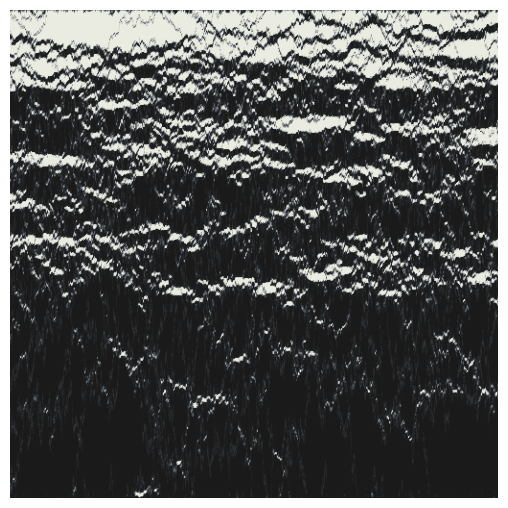
\includegraphics[width=0.24\linewidth]{../tex-src/images/flowImps/flowl0r0.png} & 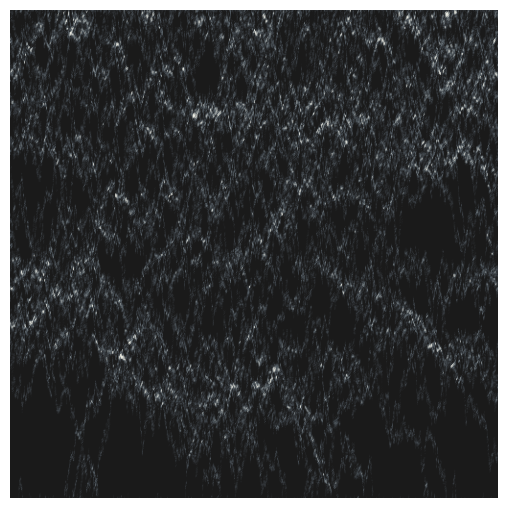
\includegraphics[width=0.24\linewidth]{../tex-src/images/flowImps/flowl1r0.png}  & 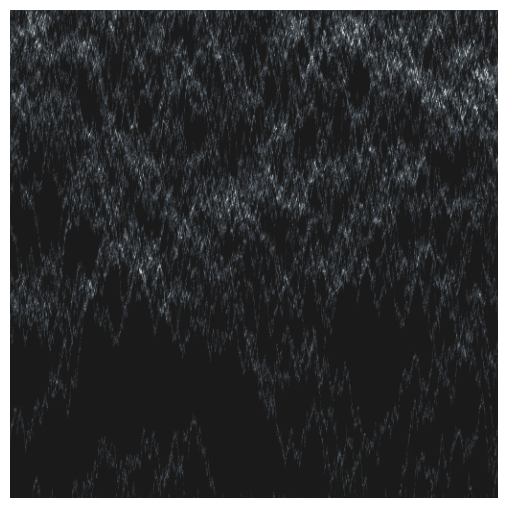
\includegraphics[width=0.24\linewidth]{../tex-src/images/flowImps/flowl2r0.png} & 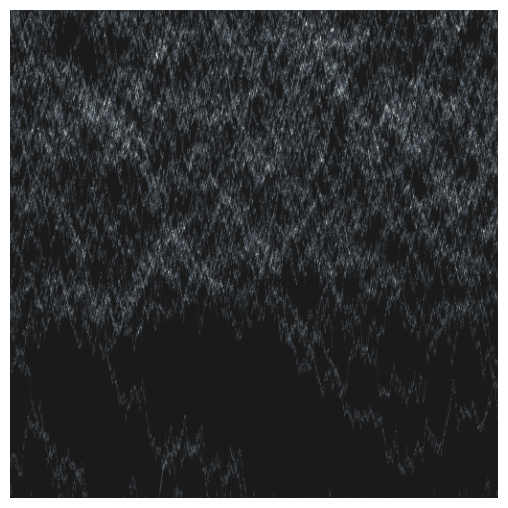
\includegraphics[width=0.24\linewidth]{../tex-src/images/flowImps/flowl3r0.png} \\
   \begin{tabular}{c} \vspace{-12em} \\ \hspace{-1em}$\rho_M=0.35$\hspace{0em} \\  \\ \end{tabular} & 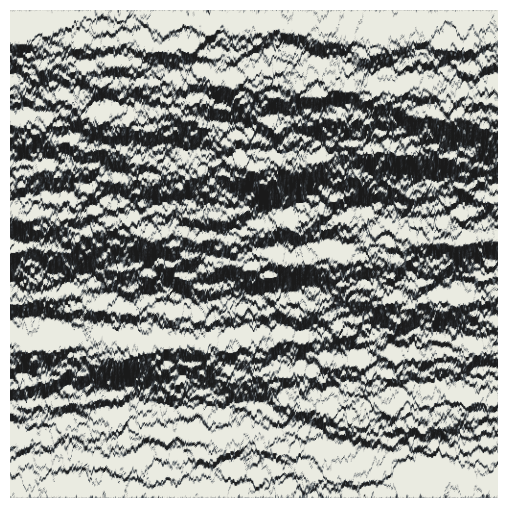
\includegraphics[width=0.24\linewidth]{../tex-src/images/flowImps/flowl0r1.png} & 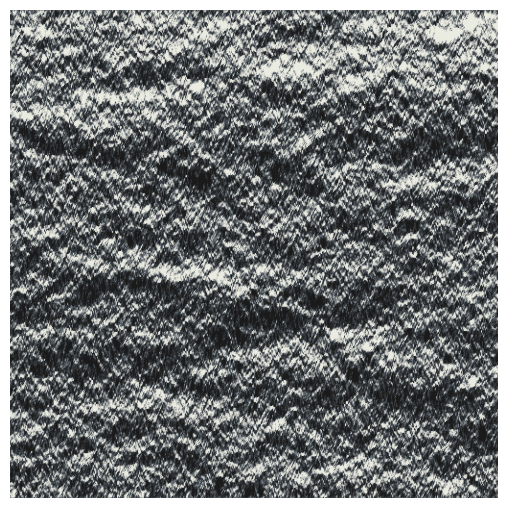
\includegraphics[width=0.24\linewidth]{../tex-src/images/flowImps/flowl1r1.png}  & 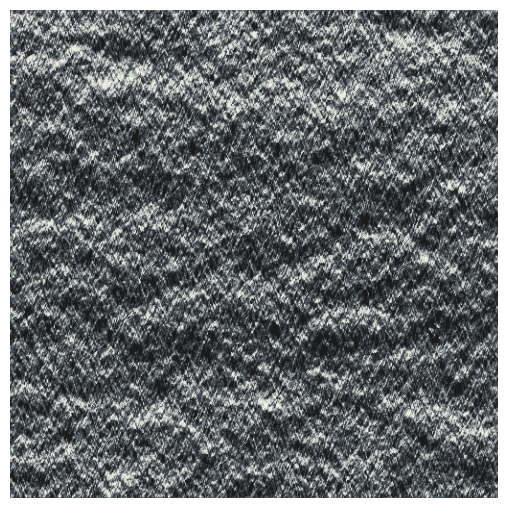
\includegraphics[width=0.24\linewidth]{../tex-src/images/flowImps/flowl2r1.png} & 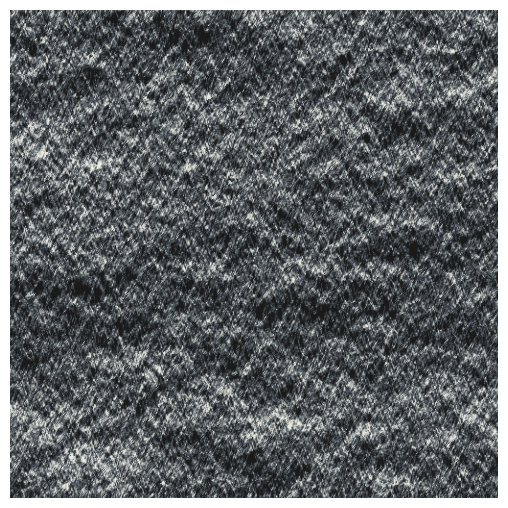
\includegraphics[width=0.24\linewidth]{../tex-src/images/flowImps/flowl3r1.png} \\
   \begin{tabular}{c} \vspace{-12em} \\ \hspace{-1em}$\rho_M=0.65$\hspace{0em} \\  \\ \end{tabular} & 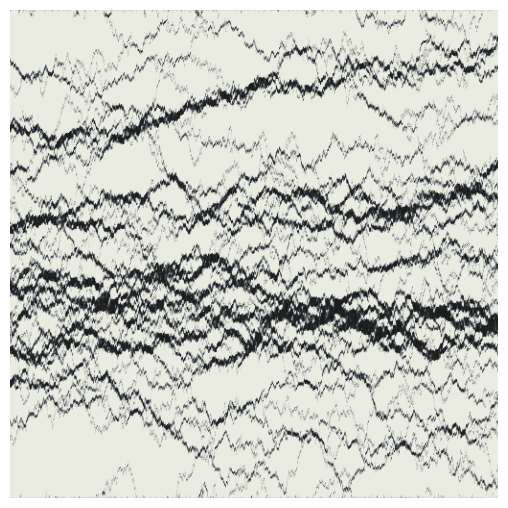
\includegraphics[width=0.24\linewidth]{../tex-src/images/flowImps/flowl0r2.png} & 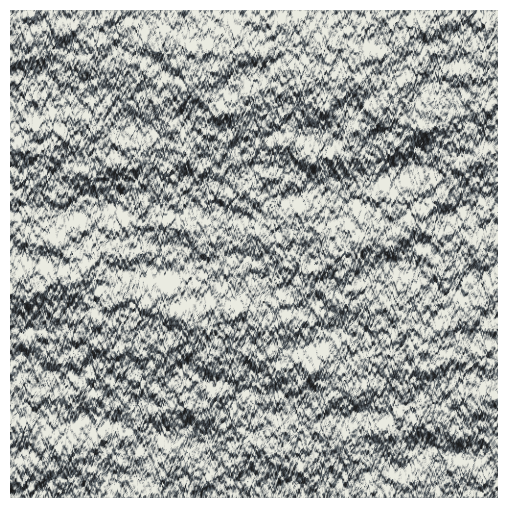
\includegraphics[width=0.24\linewidth]{../tex-src/images/flowImps/flowl1r2.png}  & 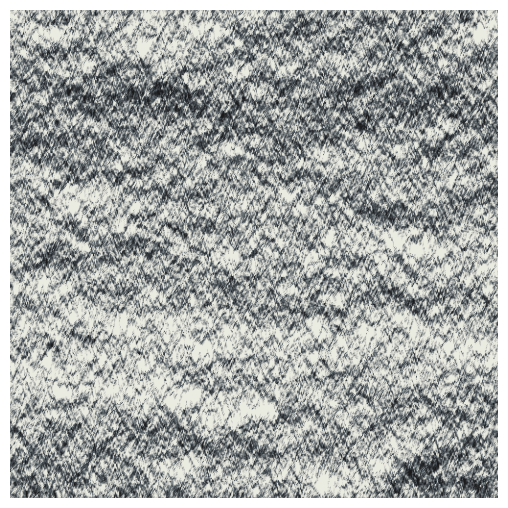
\includegraphics[width=0.24\linewidth]{../tex-src/images/flowImps/flowl2r2.png} & 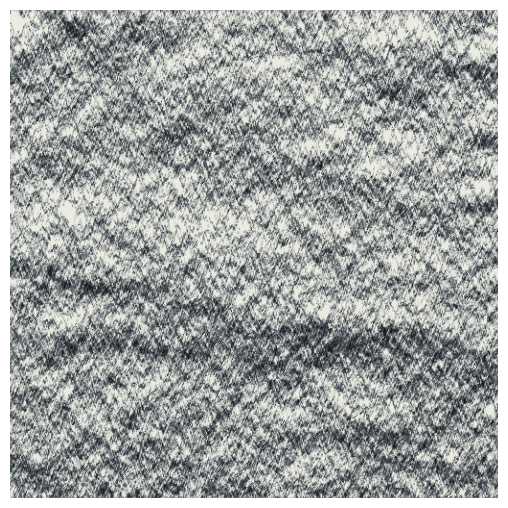
\includegraphics[width=0.24\linewidth]{../tex-src/images/flowImps/flowl3r2.png} \\
   \begin{tabular}{c} \vspace{-12em} \\ \hspace{-1em}$\rho_M=0.95$\hspace{0em} \\  \\ \end{tabular} & 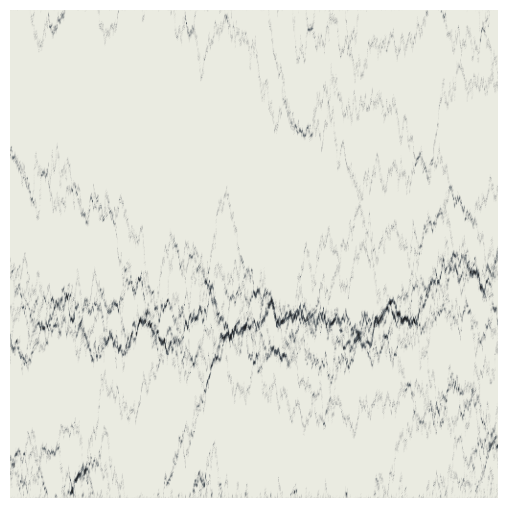
\includegraphics[width=0.24\linewidth]{../tex-src/images/flowImps/flowl0r3.png} & 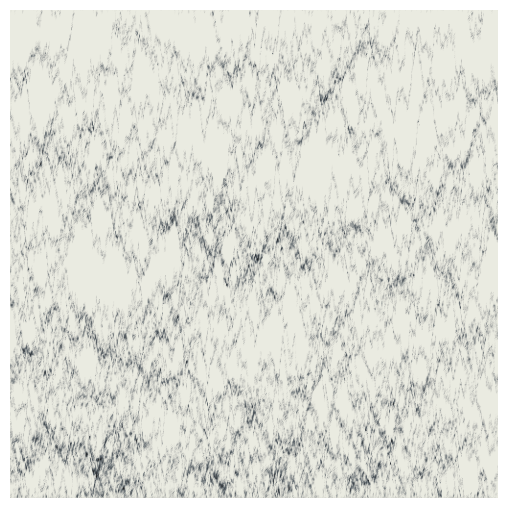
\includegraphics[width=0.24\linewidth]{../tex-src/images/flowImps/flowl1r3.png}  & 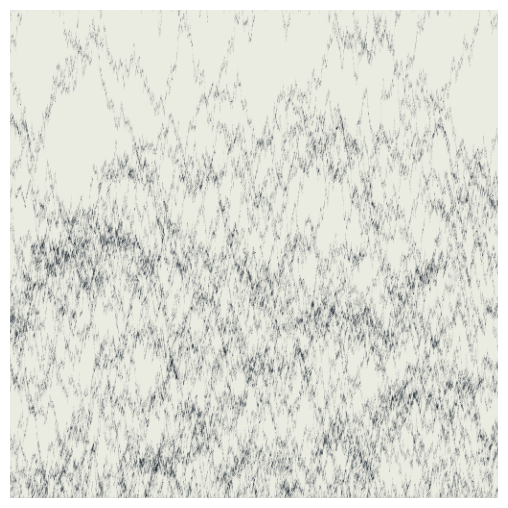
\includegraphics[width=0.24\linewidth]{../tex-src/images/flowImps/flowl2r3.png} & 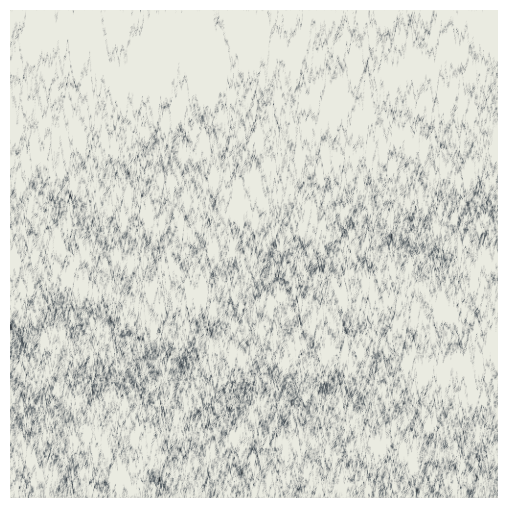
\includegraphics[width=0.24\linewidth]{../tex-src/images/flowImps/flowl3r3.png} \\
   \end{tabular}
\hspace{-1em}
&
\end{tabular}
\end{figure*}



\iffalse
\subsection{Correlation Functions}
Whilst we're calculating flow rates, we can also use our \texttt{KMCLib} code to calculate the equal time 2-point correlation function
$C(x) = \left\langle \rho(x)\rho(0) \right\rangle - \left\langle \rho(x) \right\rangle \left\langle \rho(0) \right\rangle $.
We can calculate the same quantity in a finite periodic ring analytically, and in both the analytic and numerical cases we may attempt to extract a correlation length by (curve-fitting / Laplace transform);
hence we can check whether having a steady flow through the system causes any structural effects.}
\fi

\bibliography{jHellSpring2017}



\iffalse

\section{\label{sec:level1}First-level heading}

This sample document demonstrates proper use of REV\TeX~4.1 (and
\LaTeXe) in mansucripts prepared for submission to APS
journals. Further information can be found in the REV\TeX~4.1
documentation included in the distribution or available at
\url{http://authors.aps.org/revtex4/}.

When commands are referred to in this example file, they are always
shown with their required arguments, using normal \TeX{} format. In
this format, \verb+#1+, \verb+#2+, etc. stand for required
author-supplied arguments to commands. For example, in
\verb+\section{#1}+ the \verb+#1+ stands for the title text of the
author's section heading, and in \verb+\title{#1}+ the \verb+#1+
stands for the title text of the paper.

Line breaks in section headings at all levels can be introduced using
\textbackslash\textbackslash. A blank input line tells \TeX\ that the
paragraph has ended. Note that top-level section headings are
automatically uppercased. If a specific letter or word should appear in
lowercase instead, you must escape it using \verb+\lowercase{#1}+ as
in the word ``via'' above.

\subsection{\label{sec:level2}Second-level heading: Formatting}

This file may be formatted in either the \texttt{preprint} or
\texttt{reprint} style. \texttt{reprint} format mimics final journal output. 
Either format may be used for submission purposes. \texttt{letter} sized paper should
be used when submitting to APS journals.

\subsubsection{Wide text (A level-3 head)}
The \texttt{widetext} environment will make the text the width of the
full page, as on page~\pageref{eq:wideeq}. (Note the use the
\verb+\pageref{#1}+ command to refer to the page number.) 
\paragraph{Note (Fourth-level head is run in)}
The width-changing commands only take effect in two-column formatting. 
There is no effect if text is in a single column.

\subsection{\label{sec:citeref}Citations and References}
A citation in text uses the command \verb+\cite{#1}+ or
\verb+\onlinecite{#1}+ and refers to an entry in the bibliography. 
An entry in the bibliography is a reference to another document.

\subsubsection{Citations}
Because REV\TeX\ uses the \verb+natbib+ package of Patrick Daly, 
the entire repertoire of commands in that package are available for your document;
see the \verb+natbib+ documentation for further details. Please note that
REV\TeX\ requires version 8.31a or later of \verb+natbib+.

\paragraph{Syntax}
The argument of \verb+\cite+ may be a single \emph{key}, 
or may consist of a comma-separated list of keys.
The citation \emph{key} may contain 
letters, numbers, the dash (-) character, or the period (.) character. 
New with natbib 8.3 is an extension to the syntax that allows for 
a star (*) form and two optional arguments on the citation key itself.
The syntax of the \verb+\cite+ command is thus (informally stated)
\begin{quotation}\flushleft\leftskip1em
\verb+\cite+ \verb+{+ \emph{key} \verb+}+, or\\
\verb+\cite+ \verb+{+ \emph{optarg+key} \verb+}+, or\\
\verb+\cite+ \verb+{+ \emph{optarg+key} \verb+,+ \emph{optarg+key}\ldots \verb+}+,
\end{quotation}\noindent
where \emph{optarg+key} signifies 
\begin{quotation}\flushleft\leftskip1em
\emph{key}, or\\
\texttt{*}\emph{key}, or\\
\texttt{[}\emph{pre}\texttt{]}\emph{key}, or\\
\texttt{[}\emph{pre}\texttt{]}\texttt{[}\emph{post}\texttt{]}\emph{key}, or even\\
\texttt{*}\texttt{[}\emph{pre}\texttt{]}\texttt{[}\emph{post}\texttt{]}\emph{key}.
\end{quotation}\noindent
where \emph{pre} and \emph{post} is whatever text you wish to place 
at the beginning and end, respectively, of the bibliographic reference
(see Ref.~[\onlinecite{witten2001}] and the two under Ref.~[\onlinecite{feyn54}]).
(Keep in mind that no automatic space or punctuation is applied.)
It is highly recommended that you put the entire \emph{pre} or \emph{post} portion 
within its own set of braces, for example: 
\verb+\cite+ \verb+{+ \texttt{[} \verb+{+\emph{text}\verb+}+\texttt{]}\emph{key}\verb+}+.
The extra set of braces will keep \LaTeX\ out of trouble if your \emph{text} contains the comma (,) character.

The star (*) modifier to the \emph{key} signifies that the reference is to be 
merged with the previous reference into a single bibliographic entry, 
a common idiom in APS and AIP articles (see below, Ref.~[\onlinecite{epr}]). 
When references are merged in this way, they are separated by a semicolon instead of 
the period (full stop) that would otherwise appear.

\paragraph{Eliding repeated information}
When a reference is merged, some of its fields may be elided: for example, 
when the author matches that of the previous reference, it is omitted. 
If both author and journal match, both are omitted.
If the journal matches, but the author does not, the journal is replaced by \emph{ibid.},
as exemplified by Ref.~[\onlinecite{epr}]. 
These rules embody common editorial practice in APS and AIP journals and will only
be in effect if the markup features of the APS and AIP Bib\TeX\ styles is employed.

\paragraph{The options of the cite command itself}
Please note that optional arguments to the \emph{key} change the reference in the bibliography, 
not the citation in the body of the document. 
For the latter, use the optional arguments of the \verb+\cite+ command itself:
\verb+\cite+ \texttt{*}\allowbreak
\texttt{[}\emph{pre-cite}\texttt{]}\allowbreak
\texttt{[}\emph{post-cite}\texttt{]}\allowbreak
\verb+{+\emph{key-list}\verb+}+.

\fi

\end{document}
%
% ****** End of file apssamp.tex ******
